%
%  hubcheck.tex  2012-04-09  Derrick Kearney
%
%  Describe what hubcheck is and the pieces that make it up.
%

\chapter{HUBCHECK}
\label{chap:hubcheck}


%\1 The HUBcheck Library
%  \2 HUBcheck Web Tools
%    \3 HUBcheck Webdriver Object
%      \4 Interface between HUBcheck python library and Selenium
%         Webdriver python library and ultimately Selenium Webdriver
%         and Web Browser.
%      \4 Controls setting up the web browser, connecting browser to web proxy
%      \4 Object is passed to to all web tools
%    \3 HUBcheck Web Widgets
%      \4 Reusable classes that represent bits of web pages that reoccur
%         across the hub sites.
%      \4 Classes have configurable locators
%    \3 HUBcheck Web Page Objects
%      \4 Built on top of the web widgets
%      \4 Adds web page decoration functions
%    \3 HUBcheck Web Actions
%      \4 Provide convenience functions for common actions performed by users
%      \4 Logging into website
%      \4 Creating a support ticket
%      \4 Creating a group
%      \4 Adding a wiki page to a group
%      \4 Registering a simulation tool
%  \2 HUBcheck Shell Tools
%    \3 SSH tools based on the Paramiko library
%    \3 SSHShell, SSHClient, and SFTPClient classes are thin layers
%       over the Paramiko library.
%      \4 SSHShell class provides an Expect like interface for
%         sending and receiving shell commands through an SSH
%         tunnel.
%      \4 SSHClient allows users to setup an SSHShell with their own
%         host, username, and password or key
%      \4 SFTPClient allows users to setup an SFTP client with their
%         own host, username, and password or key
%  \2 HUBcheck Other Classes
%    \3 Testdata Class
%      \4 Testdata is static information used by tests.
%      \4 Files hold account information for setting up and using
%         test accounts, web widget locators.
%      \4 Files are encrypted using AES encryption and 256 bit keys.
%    \3 TestCase Class
%      \4 Special testcase class used by HUBcheck tests, derived from Unittest.
%      \4 Automatically sets up many features standard to all HUBcheck tests
%      \4 Removes boilerplate cruft from user written test cases.
%    \3 Container Manager Class
%    \3 Proxy Class
%    \3 Tool Base Class
%\1 HUBcheck Tools
%  \2 HUBcheck Test Runner
%  \2 nanoHUB-U Enroll
%  \2 RegisterAccount
%  \2 RenderDiff
%  \2 Contribtool Automation Tools
%    \3 contribtool\_register.py
%    \3 contribtool\_upload.py
%    \3 contribtool\_install.py
%    \3 contribtool\_publish.py
%  \2 Testdata Tools
%    \3 tdedit - edit testdata files
%    \3 tdpwc - update passwords for accounts in testdata files
%\1 HUBcheck Tests
%  \2 HUBcheck unit tests
%  \2 Tool Session Container Tests
%    \3 Container configuration
%    \3 Container firewall
%    \3 Container packages
%    \3 Rappture setup and API
%    \3 Submit local and grid computing
%    \3 Webdav
%%    \3 Visualization
%  \2 Website Tests
%    \3 Support Tickets - Need Help
%    \3 Support Ticket - Report Problems
%    \3 Members Dashboard
%    \3 Website Login
%    \3 Website Redirects
%    \3 Website Tags
%    \3 Website Groups
%\end{outline}


\section{What is HUBcheck?}
\label{sec:what_is_hubcheck}

HUBcheck is a Python based library that allows users to build and run
automation tools that involve HUBzero software. While the most obvious use of
the HUBcheck library is for testing the hub website and tool session
containers, the software is designed for the more general purposes of
automating tasks that involve a web browser or an SSH shell. In the past, the
HUBcheck library has been used to enroll students into courses on the hub,
submitting support tickets, and performing hub maintenance tasks.

The goal of the HUBcheck library is to provide interfaces that interact with
HUBzero products in the same way a user would. In essence, HUBcheck mimics
a user's experience, either on the command line, or in the web browser. Using
the HUBcheck library, automation tasks can be written at a higher level,
abstracting away many of the differences between the hubs hosted by the HUBzero
Team, whether they are site design differences or HUBzero software version
differences.

\begin{figure}[tbh]
  \centering
  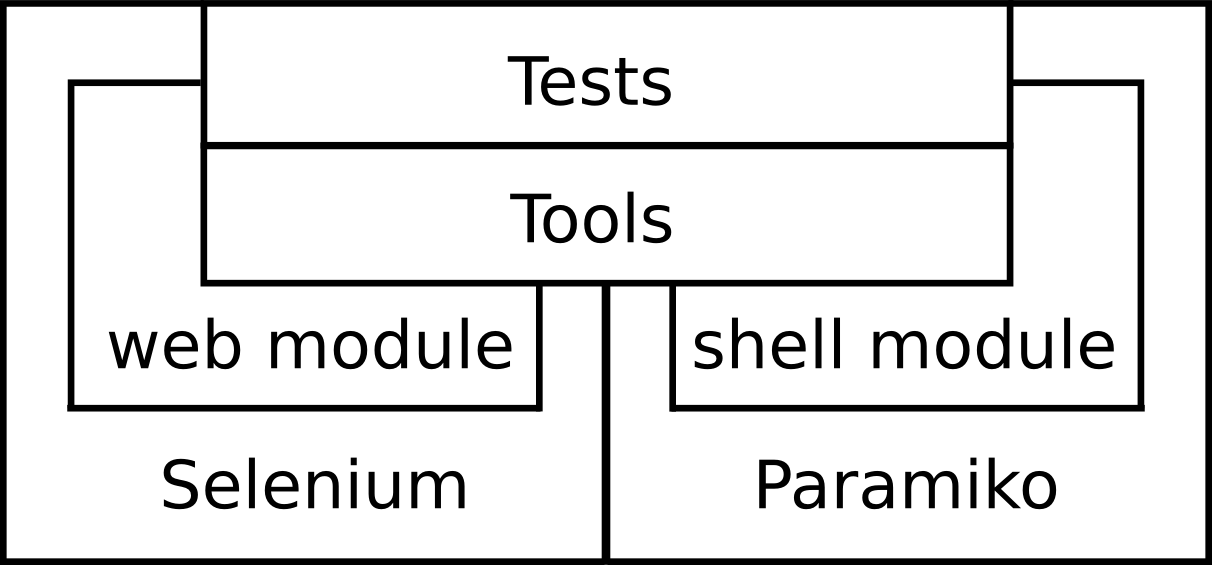
\includegraphics[width=0.5\textwidth]
    {../../images/hubcheck_block_diagram/hubcheck_library_overview_base.png}
  \caption{ The HUBcheck library builds on top of the Selenium and Paramiko libraries. }
  \label{fig:hubzero_library_overview_base}
\end{figure}

The HUBcheck library uses pseudo terminals and web browsers to perform tasks.
Pseudo terminal communication is managed by the \xfmodule{subprocess} and
\xfmodule{paramiko} modules from the Python programming language, while web
browser control is routed through Selenium WebDriver's Python bindings.  The
\xfmodule{hubcheck} package provides web modules and shell modules to perform
many of the redundant tasks required to setup the resources needed to perform
automated tasks.

\section{HUBcheck Web Modules}
\label{sec:hubcheck_web_modules}

\begin{figure}[tbh]
  \centering
  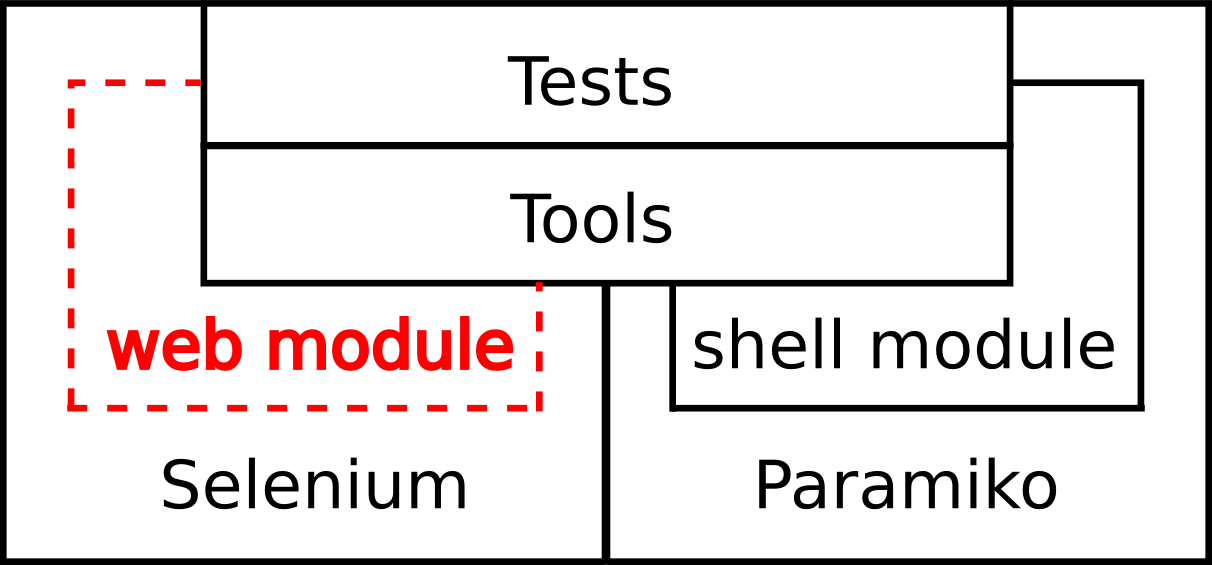
\includegraphics[width=0.5\textwidth]
    {../../images/hubcheck_block_diagram/hubcheck_library_overview_web_module.png}
  \caption{ The HUBcheck library web module can be used to launch browsers and interact with web pages. }
  \label{fig:hubzero_library_overview_web_module}
\end{figure}

HUBcheck relies upon the web browser automation of Selenium WebDriver to manage
tasks being performed on hub websites. Selenium WebDriver provides an abstract
way of controlling a number of different web browsers including Firefox,
Chrome, IE, Safari, and Opera. The most recent releases of HUBcheck support
instantiating a Firefox web browser using the \xfclass{Firefox} class. Once a
web browser has been launched, users can begin to interact with web pages using
HUBcheck's page objects, which provide common functionality for pieces of web
pages.


Consider the use case where an automation script needs to login to the hub
website as a user. In order to complete this task, the script must first launch
a web browser that can be automated. Next the script needs to tell the web
browser to navigate to the hub's login page. Once on the login page, the script
has to fill in the username and password fields, and press the login button.
Finally, the script should check that the login was successful.
\Cref{lst:selenium_ide_hubzero_login} laid out a fragile way to do this with
hard coded web element locators that were embedded inside of the automation
script. This made the script hard to read and difficult to update. An
alternative way to solve the problem, using the HUBcheck library, is shown in
\Cref{lst:hubcheck_hubzero_login}.

\begin{xcode}{%
  language=Python,%
  label=lst:hubcheck_hubzero_login,%
  caption={Login to the hubzero.org website using the HUBcheck library}%
}
import hubcheck

username = 'user1'
password = 'pass1'

hc = hubcheck.Hubcheck(hostname='hubzero.org',
                       locators='hubzero',
                       browsertype='Firefox')

# setup a web browser
hc.browser.get('https://hubzero.org')

# login to the website
po = hc.catalog.load_pageobject('LoginPage')
po.goto_page()
po.login_as(username,password)

# check that the user is logged in
po = hc.catalog.load_pageobject('GenericPage')
assert po.is_logged_in() is True
\end{xcode}

\Cref{lst:hubcheck_hubzero_login} contains no web element locators
directly in the automation script. Instead, it takes advantage of the page
objects that are a part of the HUBcheck library, which makes for a simplified
script that is easy to read and understand.
\Cref{lst:hubcheck_hubzero_login} starts, on line 6, by creating a
\xfclass{Hubcheck} object.  The \xfclass{Hubcheck} object manages both the web
browser and the page objects used in the script. Next, on line 11, the script
uses the \xfclass{Hubcheck} object to launch the web browser and navigate it to
the hub's website. To get to the hub's login page, we load the
\xfclass{LoginPage} page object on line 14 and use its \xfmethod{goto\_page()}
method to handle the navigation. Once on the login page, we employ the page
object's \xfmethod{login\_as()} method to perform the login service of filling in
the username and password fields, and clicking the login button. Lastly, the
script checks that the user was properly logged in by calling the
\xfmethod{is\_logged\_in()} method available in all HUBcheck page objects.

The sections below describe the details of opening a web browser, navigating
the hub, and using the services available through HUBcheck page objects.

\subsection{Configuring HUBcheck}
\label{ssec:hubcheck_web_modules_configure}

HUBcheck supports multiple versions of the HUBzero software, so it is important
that HUBcheck is configured properly before starting the web automation. The
most basic configuration tells HUBcheck the type of web element locators to use
and the URL of the hub where automation will occur. These two pieces of
information can be fed into the \xfclass{Hubcheck} object as parameters during
initialization.

\begin{xcode}{%
  language=Python,%
  label=lst:hubcheck_object_initialization,%
  caption={Configuring a Hubcheck object}%
}
hc = hubcheck.Hubcheck(hostname='hubzero.org',
                       locators='hubzero',
                       browsertype='Firefox')
\end{xcode}

\Cref{lst:hubcheck_object_initialization} demonstrates how to create and
configure a \xfclass{Hubcheck} object. The object allows developers to
configure the hostname of the hub under automation, the page objects that
should be used during automation, and the web browser to automate. The HUBcheck
library has page objects and web element locators from 19 of the hubs managed
by the HUBzero Team, as well as a few of the latest open source
releases. Popular locators to use include \xflocator{hubzero}, for the hubzero.org
website, and \xflocator{osr\_1\_3\_0}, for the open source release available at
the time of writing.

% Not all pages on the hub have page objects available to them.

The \xfclass{Hubcheck} object is a thin layer over three much more powerful
objects, the browser object, the catalog object and the utils object. The next
few sections discuss how these three objects are used while building HUBcheck
based web automation tools.

\subsection{Launching a Browser With the Browser Object}
\label{ssec:hubcheck_web_modules_launch_browser}

HUBcheck provides classes, representing each of the supported web browsers, to
make launching a web browser simple and fast.  The browser classes build upon
Selenium WebDriver browser objects, setting up preferences, loading browser
extensions helpful for debugging, and attaching the browser to a proxy for HTTP
response inspection.  When a \xfclass{Hubcheck} object is created, it includes
a browser object that can be used to launch a web browser by calling the
\xfmethod{get()} method.

\begin{xcode}{%
  language=Python,%
  label=lst:hubcheck_object_launch_browser,%
  caption={Launching a Firefox web browser using the Hubcheck object}%
}
hc.browser.get('https://hubzero.org')
\end{xcode}

The type of browser launched is controlled by the \xfparameter{browsertype}
argument of the \xfclass{Hubcheck} object's initialization. If no browsertype
is set, the object defaults to launching a Firefox web browser.

Behind the scenes, the \xfclass{Hubcheck} object is calling HUBcheck's
\xfclass{Firefox} class. The \xfclass{Firefox} class is responsible for setting
up the browser profile, attaching the browser to a web proxy, and launching the
browser. The same class could be called, directly by the developer, to get a
stand-alone browser object as shown in \Cref{lst:hubcheck_launch_browser}.

\begin{xcode}{%
  language=Python,%
  label=lst:hubcheck_launch_browser,%
  caption={Launching a stand-alone Firefox web browser using HUBcheck's \xfclass{Firefox} class}%
}
browser = hubcheck.browser.Firefox()
browser.get('https://hubzero.org')
\end{xcode}

\subsection{Navigating the Hub With the Catalog Object}
\label{ssec:hubcheck_web_modules_navigation}

The HUBcheck library provides page objects that express the services available
on hub web pages. Automation developers can use these page objects to ease
navigation through the hub website, perform tasks on hub web pages, or to build
new page objects using HUBcheck's widgets.

The HUBcheck library's page objects are contained within Python modules.
Additionally, each hub has a module defining which page objects work with the
hub.  These modules are accessible through the \xfobject{hubcheck} object's
\xfattribute{catalog} attribute, which is an instance of the
\xfclass{PageObjectCatalog} class.  Through the \xfattribute{catalog} attribute's
\xfmethod{load\_pageobject()} method, users instantiate new page objects
appropriate for the hub being automated.

\begin{xcode}{%
  language=Python,%
  label=lst:load_hubcheck_page_object,%
  caption={Loading a HUBcheck page object for hub navigation}%
}
# load the LoginPage page object
po = hc.catalog.load_pageobject('LoginPage')
po.goto_page()
po.login_as('testuser','pass123')
\end{xcode}

\Cref{lst:load_hubcheck_page_object} shows an example of loading the
\xfclass{LoginPage} page object, for the login web page, and assigning it to the
variable \xfparameter{po} in line 2. The script goes on to call the page object's
\xfmethod{goto\_page()} method, which is a general page object service for
navigation, and the \xfmethod{login\_as()} method, which represent a service
available on the login web page. The login web page offers several other
services like navigating to the username remind page, navigating to the
password reset page, navigating to the hub registration page, and submitting a
support ticket. All of these services are available through methods of the
LoginPage page object.


% FIXME: need to talk about the utils class
%        can mention that some of the more common actions have been made available
%        as a single method call to the utils class, like the login_as() method
%        listed above.

\subsection{Performing Common Tasks With the Utils Object}
\label{ssec:hubcheck_web_modules_common_tasks}

Automation scripts often contain repeated bits of code that perform common
tasks like logging into a website or uploading a resource. Many times the code
required to perform these tasks is copied between scripts. For large tasks,
copying code between scripts reduces code maintainability.  The HUBcheck
library provides developers with the \xfobject{utils} object which holds
functions for commonly performed tasks related to user accounts, support
tickets, and tool resource contribution.


\begin{xcode}{%
  language=Python,%
  label=lst:hubcheck_utils_login,%
  caption={Common hub tasks are made easier using the methods from the utils object}%
}
import hubcheck

username = 'user1'
password = 'pass1'

hc = hubcheck.Hubcheck(hostname='hubzero.org',
                       locators='hubzero',
                       browsertype='Firefox')

# setup a web browser
hc.browser.get('https://hubzero.org')

# login to the website
hc.utils.account.login_as(username,password)

# check that the user is logged in
po = hc.catalog.load_pageobject('GenericPage')
assert po.is_logged_in() is True
\end{xcode}

Previously, \Cref{lst:hubcheck_hubzero_login} demonstrated using the
\xfclass{LoginPage} page object and its \xfmethod{login\_as()} method to fill
in and submit the hub login form. Logging into a hub website is such a
frequently performed task, it was included as a part of the \xfclass{utils}
class. In \Cref{lst:hubcheck_utils_login}, the code that used to load
the \xfclass{LoginPage} page object, navigate to the login web page, and fill
in the login form has been replaced with a call to
\xfmethod{hc.utils.account.login\_as()}.


\section{HUBcheck Shell Modules}
\label{sec:hubcheck_shell_modules}

\begin{figure}[tbh]
  \centering
  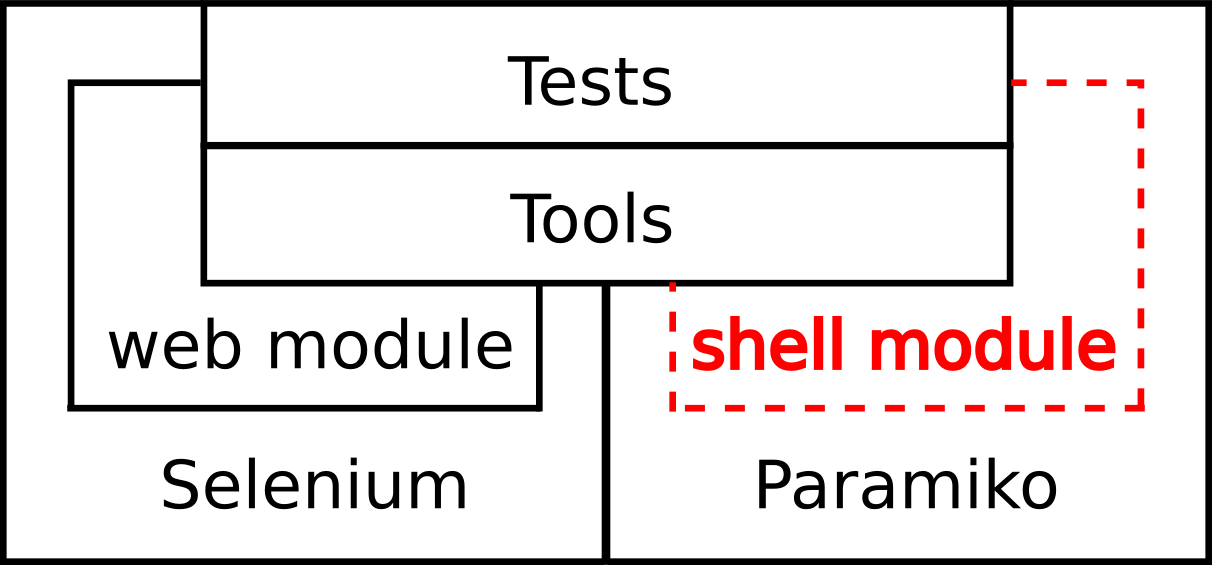
\includegraphics[width=0.5\textwidth]
    {../../images/hubcheck_block_diagram/hubcheck_library_overview_shell_module.png}
  \caption{ The HUBcheck library shell module can be used to SSH into systems and interact through the command line. }
  \label{fig:hubzero_library_overview_shell_module}
\end{figure}

The HUBcheck library also supports automation of shell utilities that run over
Secure SHell Version 2 (SSHv2), the protocol used to create encrypted channels
to services hosted on remote machines. The HUBcheck library allows developers
to quickly open interactive shells and \xfprogramname{sftp} sessions for
accessing remote hosts, including the tool session container on the hub.

% Remote Shell Access
% |-hubcheck.SSHClient
%   |-hubcheck.SSHShell
% |-hubcheck.ContainerManager
%   |-hubcheck.ToolSession
%     |-hubcheck.ToolSessionShell
% Remote File Transfer
% |-hubcheck.SFTPClient
\subsection{Starting a Remote SSH Session}
\label{ssec:starting_remote_ssh_session}

The \xfclass{hubcheck.SSHClient} class can be used to start an SSH session. The
class allows for two ways to login to the remote host, either by providing a
username and password or by providing a username and key filename, where the
key filename is a file, or list of filenames, of private keys for SSH
authentication.


\begin{xcode}{%
  language=Python,%
  label=lst:ssh_client_object,%
  caption={Connecting to a remote host over SSH}%
}
import hubcheck

sh = hubcheck.SSHClient(host='hubzero.org',
                        username='testuser',
                        password='pass123')
\end{xcode}

Upon successful authentication, an \xfclass{SSHShell} object is returned. The
\xfclass{SSHShell} object can be used to interact with the shell in a manner
similar to Expect by using calls to \xfmethod{send()} and \xfmethod{expect()}
methods.  The \xfmethod{send()} method is used to run commands over the remote
channel. It accepts a single parameter, the command to be run. The
\xfmethod{expect()} method is used to retrieve output from the remote channel's
buffer. It accepts a list of patterns and tries to match each pattern to the
data in the channel's buffer.  If it finds a match, the matching data is stored
and the method returns the index of the pattern that matched the data.
\Cref{lst:ssh_shell_send_expect} shows examples of using the \xfmethod{send()}
and \xfmethod{expect()} methods.

\begin{xcode}{%
  language=Python,%
  label=lst:ssh_shell_send_expect,%
  caption={Using the Expect like interface of SSHShell}%
}
sh.send('echo hi')
r = sh.expect('hi')
# r == 0, the index of the matched pattern 'hi'

sh.send('echo hi')
r = sh.expect(['tie','hi','bye',sh.TIMEOUT])
# r == 1, the index of the matched pattern 'hi'

sh.send('echo hi')
r = sh.expect(['cry',sh.TIMEOUT])
# r == -1, no patterns matched, expect() timed out
\end{xcode}

The \xfmethod{expect()} method uses Python's regular expression module,
\xfmodule{re}, and can accept complicated regular expressions as patterns. If
the pattern argument contains a regular expression that is matched to data in
the channel's buffer, the resulting \xfobject{re.match} object is stored in the
SSHShell object's \xfparameter{match} attribute, where the developer can query
it further for the exact text and groupings that were matched.
\Cref{lst:ssh_shell_expect_match} shows how to access matches found by the
\xfmethod{expect()} method.

\begin{xcode}{%
  language=Python,%
  label=lst:ssh_shell_expect_match,%
  caption={Using a regular expression as a pattern in the expect() method}%
}
# grab the prompt and escape it for use in a regular expression
import re
prompt = re.escape(sh.get_prompt())

# match any string
sh.send('echo hi')
sh.expect(['(.*){0}'.format(prompt)])
# the matching text is stored in a re.match object, available through sh.match
result = sh.match.groups()[0]
# result == 'hi\r\n'
\end{xcode}


\subsection{Accessing a Hub's Tool Session Container Using SSH}
\label{ssec:hubcheck_shell_modules_accessing_container_ssh}

Tool session containers on the hub can be accessed via an SSH connection, but
SSH'ing into one can be a little tricky due to the hub configuration. All
connections to the hub are routed through the the hub's web server, including
connections destined for the web server and connections destined for tool
session containers. For example, on the imaginary hub named
\xfhtmllink{myhub.org}, a developer, with elevated permissions to login
directly on the web server, would use the command shown in
\Cref{lst:ssh_hub_webserver} to login to the hub's web server.

\begin{xcode}{%
  language=bash,%
  label=lst:ssh_hub_webserver,%
  caption={SSH'ing into a hub's webserver}%
}
ssh user@myhub.org
\end{xcode}

In order to SSH into a tool session container hosted on the hub, the developer
needs to use the hub's VirtualSSH proxy interface provided by the
\xfprogramname{session} command, as shown in
\Cref{lst:ssh_hub_container}.

\begin{xcode}{%
  language=bash,%
  label=lst:ssh_hub_container,%
  caption={SSH'ing into a hub's tool session container}%
}
ssh -t -X user@myhub.org session
\end{xcode}

Normal users, without the elevated permissions needed to login on the web
server, could use either command to connect to the hub, but in the case of
\Cref{lst:ssh_hub_webserver}, the request would be automatically
forwarded into a tool session container.

HUBcheck provides the \xfclass{ToolSession} class to help developers connect to
tool session containers through the hub's VirtualSSH proxy. The
\xfclass{ToolSession} class offers methods analogous to commands of the
VirtualSSH proxy including the ability to start, stop, access, and list
available tool session containers for a user with a password.
\Cref{tab:virtualSSHToolSession} outlines the equivalent ToolSession methods for
each of the Virtual SSH commands.

\begin{table}
  \centering
  \caption{HUBcheck's ToolSession class gives developers easy access to the
           hub's Virtual SSH Commands.}
  \begin{tabular}{ l | l }
    \hline
    ssh [flags] [user@]hostname [command] & ts = ToolSession( \\
                                          &   host,port,username,password) \\
                                          &                       \\
                                          &                       \\ \hline
    Virtual SSH Commands                  & ToolSession Object Methods \\ \hline
                                          &                       \\
    session create [session\_title]       & create(title=None)    \\
                                          &                       \\
    session start                         & start()               \\
                                          &                       \\
    session [session\_number] [command]   & access(snum=None,command=None) \\
                                          &                       \\
    session list                          & list()                \\
                                          &                       \\
    session stop session\_number          & stop(session\_number) \\
                                          &                       \\
    session help                          & help()                \\
                                          &                       \\
    \hline
  \end{tabular}
  \label{tab:virtualSSHToolSession}
\end{table}


\subsubsection{Starting a Tool Session Container With HUBcheck}
\label{ssec:hubcheck_shell_modules_starting_container}

VirtualSSH provides two ways to start a tool session container, using the
\xfprogramname{session create} or \xfprogramname{session start} subcommands.
The \xfprogramname{session create} subcommand initiates the creation of a tool
session container, allowing the developer to name the container by setting the
\xfparameter{session\_title} parameter.  After calling the
\xfprogramname{session create} subcommand, the user is returned to their local
shell with a session number they can connect to.  Similarly, the
\xfprogramname{session start} subcommand also initiates the creation of a tool
session container, but goes the extra step of placing the user into the
container where they can run shell commands on the remote host.

\begin{xcode}{%
  language=bash,%
  label=lst:virtualssh_start_tool_session_container,%
  caption={Starting a hub tool session container using VirtualSSH}%
}
ssh user@myhub.org session create
# 40023, a session number is returned to the user

ssh user@myhub.org session create mytitle
# 40023, a session number is returned to the user

ssh user@myhub.org session start
# user is placed into the tool session container
\end{xcode}

HUBcheck's \xfclass{ToolSession} class provides access to these subcommands
through the \xfmethod{create()} and \xfmethod{start()} methods. Just like
VirtualSSH's \xfprogramname{session create} subcommand, the \xfmethod{create()}
method accepts an optional session title, but it returns three Paramiko
\xfclass{ChannelFile} objects that can be treated like Python file objects. One
of the \xfclass{ChannelFile} objects, \xfparameter{stdout}, holds the session
number of the newly created session. The \xfclass{ToolSession} class's
\xfmethod{start()} method accepts no arguments and returns a
\xfclass{ToolSessionShell} object, which is derived from the \xfclass{SSHShell}
class introduced in \Cref{ssec:starting_remote_ssh_session}.
\Cref{lst:toolsession_start_tool_session_container} shows how to create and
start tool session containers using HUBcheck's \xfclass{ToolSession} class.

\begin{xcode}{%
  language=python,%
  label=lst:toolsession_start_tool_session_container,%
  caption={Starting a hub tool session container using the ToolSession class}%
}
import hubcheck

ts = hubcheck.ToolSession(hostname,
                          username = username,
                          password = password)

(stdin,stdout,stderr) = ts.create()
# stdout.read() provides the session number

(stdin,stdout,stderr) = ts.create('mytitle')
# stdout.read() provides the session number

shell = ts.start()
# shell is a ToolSessionShell, a type of SSHShell
\end{xcode}


\subsubsection{Accessing a Tool Session Container With HUBcheck}
\label{ssec:hubcheck_shell_modules_accessing_container}

The default behavior of VirtualSSH's \xfprogramname{session} command is to
place the user into a tool session container.  If the developer has multiple
tool session containers running, they can choose which one to enter by
providing the \xfprogramname{session} command with an integer argument
representing the  session number, a unique integer identifier for a tool
session container. The \xfprogramname{session} command also accepts an optional
\xfparameter{command} argument.  When the \xfparameter{command} argument is
provided, \xfprogramname{session} will execute the command in the tool session
container and return the user to the local shell along with the stdout and
stderr streams from the command.
\Cref{lst:virtualssh_access_tool_session_container} shows how VirtualSSH's
\xfprogramname{session} command can be used to get into a tool session
container with no arguments, with a session number, and with a command.

\begin{xcode}{%
  language=bash,%
  label=lst:virtualssh_access_tool_session_container,%
  caption={Accessing a hub tool session container using VirtualSSH}%
}
ssh user@myhub.org session
# user is placed into an open tool session container

ssh user@myhub.org session 40023
# user is placed into tool session container with session number 40023

ssh user@myhub.org session "echo hi"
# the command "echo hi" is run in a tool session container.
# "hi" is returned to stdout, user is returned to local shell

ssh user@myhub.org session 40023 "echo hi"
# the command "echo hi" is run in the tool
# session container with session number 40023
# "hi" is returned to stdout, user is returned to local shell
\end{xcode}

The \xfclass{ToolSession} class provides tool session container access through
the \xfmethod{access()} method. The \xfmethod{access()} method accepts two
parameters, representing the session number and the command to run in the tool
session container, just like VirtualSSH's \xfprogramname{session} command.
Example use of the \xfmethod{access()} method is shown in
\Cref{lst:toolsession_access_tool_session_container}.

\begin{xcode}{%
  language=python,%
  label=lst:toolsession_access_tool_session_container,%
  caption={Accessing a hub tool session container using the ToolSession class}%
}
shell = ts.access()
# places user into a tool session container and returns
# a ToolSessionShell object to control the container.

shell = ts.access(session_number=40023)
# places user into tool session container with
# session number 40023, and returns a ToolSessionShell
# object to control the container.

(stdin,stdout,stderr) = ts.access(command='echo hi')
# runs the command 'echo hi' in a tool session container
# returns stdin, stdout, and stderr to the user.

(stdin,stdout,stderr) = ts.access(40023,'echo hi')
# runs the command 'echo hi' in  tool session container
# with session number 40023. returns stdin, stdout, and
# stderr to the user.
\end{xcode}


\subsubsection{Listing Available Tool Session Containers With HUBcheck}
\label{ssec:hubcheck_shell_modules_listing_containers}

VirtualSSH's \xfprogramname{session list} subcommand can be used to get a list of
available tool session containers for a user. For each open tool session
container, the command returns the session number, session name, and session
title. The session name is the name of the tool that started the session. This
is usually a workspace, but could be any of the installed tools on the hub
since they all run in tool session containers. The \xfprogramname{session list}
subcommand also denotes the default tool session container for SSH connections by
using a * in the output column named \texttt{Default}.
\Cref{lst:virtualssh_list_tool_session_containers} shows example output from
VirtualSSH's \xfprogramname{session list} subcommand.

\begin{xcode}{%
  language=bash,%
  label=lst:virtualssh_list_tool_session_containers,%
  caption={Listing available hub tool session containers using VirtualSSH}%
}
ssh user@myhub.org session list
#   Number  Default Name                 Title
#     8374     *    workspace_r1         Workspace (6:57 pm)
#     8584          workspace_r1         Workspace
# Connection to myhub.org closed.
# user is placed back in their local shell
\end{xcode}

This same information can be retrieved programmatically by using the
\xfmethod{list()} method in the \xfclass{ToolSession} class. Similar to running
a command in a tool session container, the \xfmethod{list()} method returns its
output as a 3-tuple whose elements represent the stdin, stdout, and stderr
channels as Python file-like objects.
\Cref{lst:toolsession_list_tool_session_containers} shows an example of using
the \xfclass{ToolSession} class's \xfmethod{list()} method.

\begin{xcode}{%
  language=python,%
  label=lst:toolsession_list_tool_session_containers,%
  caption={Listing available hub tool session containers using the ToolSession class}%
}
(stdin,stdout,stderr) = ts.list()
# returns the list of open sessions to the stdout variable

stdout.read()
#   Number  Default Name                 Title
#     8374     *    workspace_r1         Workspace (6:57 pm)
#     8584          workspace_r1         Workspace
\end{xcode}

To make accessing the information easier, the \xfclass{ToolSession} class also
provides the \xfmethod{get\_open\_session\_detail()} method, which returns the
same information as an iterable Python dictionary, with row numbers as keys and
row data as values.

\begin{xcode}{%
  language=python,%
  label=lst:toolsession_list_tool_session_containers2,%
  caption={Iterating through tool session container details}%
}
import pprint

details = ts.get_open_session_detail()
# returns a dictionary of open session data

pprint.pprint(details)
#{0: {'default': True,
#     'name': 'workspace_r1',
#     'session_number': '8374',
#     'title': 'Workspace (6:57 pm)'},
# 1: {'default': False,
#     'name': 'workspace_r1',
#     'session_number': '8584',
#     'title': 'Workspace'}}

for row in details.values():
  if row['session_number'] == '8584':
    title = row['title']

print title
# Workspace
\end{xcode}


\subsubsection{Stopping Tool Session Containers With HUBcheck}
\label{ssec:hubcheck_shell_modules_stop_containers}

VirtualSSH allows users to stop a tool session container using the
\xfprogramname{session stop} subcommand. The command accepts an integer argument that
specifies the session number that should be stopped.

\begin{xcode}{%
  language=bash,%
  label=lst:virtualssh_stop_tool_session_container,%
  caption={Stopping a hub tool session container using VirtualSSH}%
}
ssh user@myhub.org session stop 40023
# stopping session 40023
# Connection to myhub.org closed.
# user is placed back in their local shell
\end{xcode}

To stop tool session containers using the \xfclass{ToolSession} class, use the
\xfmethod{stop()} method. The \xfmethod{stop()} method accepts a single
parameter, an integer session number specifying the tool session container to
stop.

\begin{xcode}{%
  language=python,%
  label=lst:toolsession_stop_tool_session_containers,%
  caption={Stopping a hub tool session containers using the ToolSession class}%
}
(stdin,stdout,stderr) = ts.stop(40023)
\end{xcode}


\subsection{Managing Tool Session Containers}
\label{ssec:hubcheck_shell_modules_managing_containers}

When writing automated scripts and tests, keeping track of all of the tool
session containers being opened and closed can be a hassle. HUBcheck tries
address this by offering the \xfclass{ContainerManager} class, which promotes
the efficient reuse of tool session containers when possible. The
ContainerManager class is a singleton that can be used to create, access, and
stop tool session containers for multiple users.

Consider the case where several test cases need access to a tool session
container to perform a test. The simple solution would be to have each test
case start, access, and stop a new tool session container to perform its test.
This approach provides isolation between each test, helping ensure
another resource doesn't accidentally close the tool session container while a
test case is using it. It is, however, terribly inefficient. Starting up a tool session
container takes a few seconds and using it for a single, non-destructive
test would be wasteful. Often, an execution of HUBcheck runs hundreds of tests,
the majority of which only query resources in the tool session container,
leaving it in good condition for further use. The approach taken by many
HUBcheck based tools is to reuse tool session containers whenever possible.

The \xfclass{ContainerManager} class helps implement a tool session container
reuse approach. Accessing tool session containers is similar to using the
\xfclass{ToolSession} class directly, but removes most of the rarely used
features. The \xfclass{ContainerManager} class provides an \xfmethod{access()}
method developers can use to enter a tool session container. The
\xfmethod{access()} method takes three parameters, the hostname of the hub
hosting the tool session container, the username and the password of the user
opening the tool session container.  Given this information, the
\xfclass{ContainerManager} class looks in its internal dictionary to see if it
already has a tool session container open for the hostname and username
combination. If it does, a new shell for that container is opened and returned
to the user as a \xfclass{ToolSessionShell} object. If not, a new tool session
container is created and a \xfclass{ToolSessionShell} object is returned.

\begin{xcode}{%
  language=python,%
  label=lst:containermanager_access_tool_session_containers,%
  caption={Accessing a tool session container using the ContainerManager class}%
}
import hubcheck

cm = hubcheck.ContainerManager()

ws1 = cm.access(hostname,username,password)
# ws1 is a ToolSessionShell object

session_number1 = ws1.execute('echo $SESSION')
# '40023'
\end{xcode}

The \xfclass{ContainerManager} can track multiple open tool session containers,
by multiple users, on multiple hubs.  Calling the \xfmethod{access()} method a
second, or a third, time with the same hostname and username results in
additional shells being opened in the same tool session container.

\begin{xcode}{%
  language=python,%
  label=lst:containermanager_multiple_access_tool_session_containers,%
  caption={Multiple accesses to a tool session container using the ContainerManager class}%
}
ws2 = cm.access(hostname,username,password)
# ws2 is another ToolSessionShell object

session_number2 = ws2.execute('echo $SESSION')
# '40023'
\end{xcode}

Calling the \xfmethod{access()} method with a different hostname or username
results in a new tool session container being created.

\begin{xcode}{%
  language=python,%
  label=lst:containermanager_multiuser,%
  caption={ContainerManager can handle multiple users' tool session containers}%
}
ws3 = cm.access(hostname,username2,password2)
# ws3 is another ToolSessionShell object

session_number3 = ws3.execute('echo $SESSION')
# '40024'
\end{xcode}


In many HUBcheck based tools, there is little advantage to closing a tool
session container before the program ends, but for the times when this is
needed, the \xfclass{ContainerManager} class provides the \xfmethod{stop()} and
\xfmethod{stop\_all()} methods. The \xfmethod{stop()} method uses its
parameters, a hostname, username, and session number, to determine which tool
session container to stop.  The \xfmethod{stop\_all()} method loops through all
tool session containers managed by the \xfclass{ContainerMananger} object and
stops them.

\begin{xcode}{%
  language=python,%
  label=lst:containermanager_stop_tool_session_containers,%
  caption={Stopping a tool session container using the ContainerManager class}%
}
cm.stop(hostname,username,session_number)
# stop username's tool session container on host hostname
# with session number session_number

cm.stop_all()
# stop all tool session containers managed by the cm object.
\end{xcode}


\subsection{Interacting With the Tool Session Container}
\label{ssec:hubcheck_shell_modules_interacting_containers}

A \xfclass{ToolSessionShell} object is returned for many of the methods that
access a tool session container. The \xfclass{ToolSessionShell} class is
derived from the \xfclass{SSHShell} class and provides the \xfmethod{send()}
and \xfmethod{expect()} methods described in
\Cref{ssec:starting_remote_ssh_session}. It also provides the
\xfclass{SSHShell}'s \xfmethod{execute()} method, which combines both the
\xfmethod{send()} and \xfmethod{expect()} methods into one function call that
checks the exit status of the executed command. If a command returns a
non-zero exit status, an \xfclass{ExitCodeError} exception is raised, and
command execution stops. In this respect, the \xfmethod{execute()} method acts
like a shell with the \textbf{-e} flag set, where a script will exit
immediately upon error. A successful call to the \xfmethod{execute()} method
returns the output of the command and the exit status of executing the command.

\begin{xcode}{%
  language=python,%
  label=lst:toolsessionshell_execute_method,%
  caption={Interacting with the tool session container using the ToolSessionShell class}%
}
import hubcheck

cm = hubcheck.ContainerManager()

ws = cm.access(hostname,username,password)
# ws is a ToolSessionShell object

out,es = ws.execute('echo hi')

print out
# 'hi'
\end{xcode}

The \xfclass{ToolSessionShell} class provides features specific to working in the shell
of a tool session container. It provides the \xfmethod{importfile()} method to
transfer files from the user's desktop into the tool session container, the
\xfmethod{exportfile()} method to transfer files from the tool session container
to the user's desktop, and a few functions to simplify parsing tool session
container resource files.


\subsection{Transferring Files Between The User Desktop and the Hub}
\label{ssec:hubcheck_shell_modules_sftp}

The hub supports three methods of transporting files between the user desktop
and the user's hub account, including \xfurischeme{webDAV},
\xfurischeme{filexfer}, and \xfurischeme{sftp}. HUBcheck provides ways to use
\xfurischeme{filexfer} and \xfurischeme{sftp}, while the Python module
\xfmodule{webdavlib} \cite{WebDAVLib:Online} provides a reliable client-side
interface for the \xfurischeme{webDAV} \cite{WebDAV:Online} protocol.

% FIXME: \cite webdavlib
% https://launchpad.net/python-webdav-lib

% FIXME \cite webdav protocol
% https://tools.ietf.org/html/rfc4918
% https://en.wikipedia.org/wiki/WebDAV

The hub's \xfurischeme{filexfer} protocol consists of two commands,
\xfprogramname{importfile} and \xfprogramname{exportfile}. Filexfer transfers
start on the command line of a tool session container's X terminal, by issuing
the the \xfprogramname{importfile} command to transfer files from the user's
desktop into their hub account, or the \xfprogramname{exportfile} command
to transfer files from the user's hub account into their desktop. The
\xfurischeme{filexfer} commands use the tool session container's
\xfprogramname{clientaction} program to initiate a popup window in the user's
web browser. When importing a file, the user populates the popup window with
the text or filename they would like transferred into their hub account. After
submitting the form in the popup window, the data is then saved in the hub
account. When exporting a file, the popup window contains the data of the file
from the user's hub account.

To implement simple file transfers, the \xfclass{ToolSessionShell} class
provides the \xfmethod{importfile()} and \xfmethod{exportfile()} methods. Both
methods take two arguments representing a local filename from inside of the
workspace and a remote filename from the user's desktop. The direction of
transfer is determined by the method being called. Under the hood, these two
functions approximate the actions being performed by the hub's
\xfurischeme{filexfer} commands, by using the \xfurischeme{sftp} protocol to
transfer the files. It is possible to use HUBcheck's web module in coordination
with the \xfclass{ToolSessionShell} class to more closely imitate what users
would really do on the hub, but the goal of the implementation is to transfer
files and, on the command line, using \xfurischeme{sftp} is more efficient.

\begin{xcode}{%
  language=python,%
  label=lst:toolsessionshell_filexfer,%
  caption={Transferring files using ToolSessionShell's importfile and exportfile methods}%
}
import hubcheck

cm = hubcheck.ContainerManager()

ws = cm.access(hostname,username,password)
# ws is a ToolSessionShell object

# importing a file from the desktop to the hub account
ws.importfile('desktop_file.txt', 'hub_file.txt')

# importing data from the desktop to a file in the hub account
file_data = 'transferring is easy'
fsize = ws.importfile(file_data, 'hub_file.txt', is_data=True)
assert fsize == len(file_data)

# exporting a file from the hub account to the desktop
ws.exportfile('hub_file.txt', 'desktop_file.txt')

\end{xcode}

For more control over how files are transferred, the HUBcheck library also
provides access to Paramiko's \xfclass{SFTPClient} class.  HUBcheck's
\xfclass{SFTPClient} class is a small wrapper class around the Paramiko
\xfclass{SFTPClient} class, which can be used to access a user's hub account
through the \xfurischeme{sftp} protocol. With this method, users have full access
to \xfurischeme{sftp} functions like \xfmethod{get}, \xfmethod{put},
\xfmethod{remove}, \xfmethod{chmod}, \xfmethod{open}, \xfmethod{chdir}, and
more.

\begin{xcode}{%
  language=python,%
  label=lst:sftpclient,%
  caption={Transferring files using the SFTPClient class}%
}
import hubcheck

sftp = hubcheck.SFTPClient(hostname,username=username,password=password)
# sftp is a Paramiko SFTPClient object

# transfer file from the hub account to the desktop
sftp.get('hub_file.txt','desktop_file.txt')

# transfer file from the desktop to the hub account
sftp.put('desktop_file.txt','hub_file.txt')

# close the sftp connection
sftp.close()
\end{xcode}

% HUBcheck Tools
% |-tool.py
%   |-parsing command line options and config files
%     |-focus on hubcheck features:
%       hubcheck configuration file
%       logfile/loglevel
%       usage, showing, recording of virtual display
%       highlight web elements as they are searched for
%       scrolling web page to view web elements being interacted with
%       directories for screenshots and videos
%       port for running web proxy
%       smtp setting for emailing results
%   |-setup logging
%   |-xvfb setup (with window manager, and recording, and viewing)
%     |-pyvirtualdisplay is used to start the virtual display
%     |-icewm window manager also started
%     |-hub
%   |-web proxy configuration
%     |-browsermob proxy is used as the web proxy
%     |-use the port from the command line or config file option
%   |-running the command
% |-building your own tool
%   |-subclass hubcheck.Tool
%   |-adding command line or config file options
%   |-define a command() method
%   |-make your module a standalone program
% |-examples
%   |-test runner (hctestrunner)
%   |-nightly rappture builds
%     |-hcnrb.py (trunk and branch-1.3)
%     |-hcnrb_tests_lang_tcl.py
%   |-test user tools
%     |-profile update (hcuserprofile)
%     |-account registration (register_account)
%     |-password change (hcpwc)
%   |-solarpv database update (solarpv_db_update.py)

\section{Building Applications Backed by the HUBcheck Library}
\label{sec:building_hubcheck_backed_applications}

\begin{figure}[tbh]
  \centering
  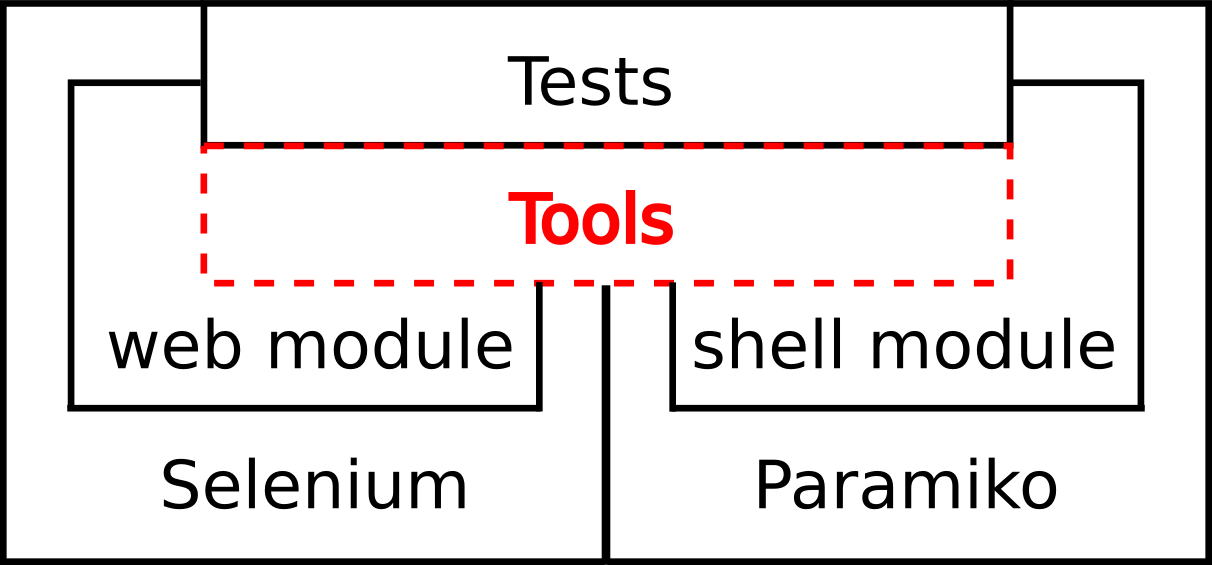
\includegraphics[width=0.5\textwidth]
    {../../images/hubcheck_block_diagram/hubcheck_library_overview_tools.png}
  \caption{ Command line utilities can be built on top of the HUBcheck %
            library by using the \xfclass{hubcheck.Tool} class. }
  \label{fig:hubzero_library_overview_tools}
\end{figure}

The HUBcheck library includes several programs that build upon the web and
shell modules. While each program has a different goal, there are features
common to all of them, like configuration options and environment setup, that
are tedious to write for one program and inefficient to copy for multiple
programs. For this reason, HUBcheck includes the \xfclass{hubcheck.Tool} class,
which can be subclassed to get a common set of command line and configuration
file options with an intuitive parser, automatic logging setup, a virtual
display for running web browser based automation, and a web proxy to help
monitor, block and analyze communications between a web browser and a web site.

Below, we explore the features of \xfclass{hubcheck.Tool} based programs by
building an example tool that performs a user login through the hub's web
and SSH interfaces.

\subsection{Building a Tool}
\label{ssec:building_a_tool}

\xfclass{hubcheck.Tool} is a base class for command line tools that use the
HUBcheck library. The class provides many of the boilerplate features that are
repeated in HUBcheck based programs. By subclassing \xfclass{hubcheck.Tool},
users can quickly create a feature rich command line tool for automating web
and shell access on the hub.

\begin{xcode}{%
  language=python,%
  label=lst:hc_tool_template,%
  caption={HUBcheck based tools follow this general template}%
}
import hubcheck

class LoginTool(hubcheck.Tool):
    def __init__(self,logfile='hcutils.log',loglevel='INFO'):
        super(LoginTool,self).__init__(logfile,loglevel)
        # introduce new command line and configuration options

        # parse command line / config file options, start logging
        self.parse_options()
        self.start_logging()

    def command(self):
        # add code that does the work

if __name__=='__main__':
    tool = LoginTool()
    tool.run()
\end{xcode}


There are three steps to creating a new HUBcheck based tool:

\begin{enumerate}
\item Subclass \xfclass{hubcheck.Tool} to create a new tool class.
\item Populate the tool's \xfmethod{\_\_init\_\_()} and \xfmethod{command()} methods.
\item Call the \xfmethod{run()} method of an instance of the tool's class.
\end{enumerate}

\noindent \Cref{lst:hc_tool_template} shows the general template for HUBcheck
based tools.  The template starts by subclassing \xfclass{hubcheck.Tool} into a
class named \xfclass{LoginTool}, the name of the tool we are creating.
\xfclass{hubcheck.Tool}'s \xfmethod{\_\_init\_\_()} method takes care of
setting up command line and configuration file option parsing, so it is
important that it is called early in the object creation process. In
\Cref{lst:hc_tool_template}, this happens in line 5. \xfclass{hubcheck.Tool}'s
\xfmethod{\_\_init\_\_()} method sets up five variables that can be used by the
\xfclass{LoginTool} class:

\begin{enumerate}
\item \xfparameter{self.command\_parser}
\item \xfparameter{self.config\_parser}
\item \xfparameter{self.options}
\item \xfparameter{self.logger}
\item \xfparameter{self.testdata}
\end{enumerate}

\noindent
The first two, \xfparameter{self.command\_parser} and \xfparameter{self.config\_parser},
are parsers for options set on the command line or in an INI-style
configuration file. You can manipulate these variables inside of
\xfmethod{\_\_init\_\_()}, using their \xfmethod{add\_argument()} and
\xfmethod{add\_option()} methods respectively, to add new options that the
parsers will recognize.

\begin{xcode}{%
  language=python,%
  label=lst:hc_tool_template_add_command_line_flag,%
  caption={Use the \xfmethod{add\_argument()} method to define new command line flags for the tool}%
}
    def __init__(self,logfile='hcutils.log',loglevel='INFO'):
        ...
        # introduce new command line and configuration options
        self.command_parser.add_argument(
            '--video-filename',
            help='name of the video file',
            action="store",
            dest="videofn",
            default='password_change.mp4',
            type=str)
        ...
\end{xcode}

The \xfclass{hubcheck.Tool} class includes functionality to record the virtual
display where the web browser window is running, but does not expose the
ability to name the file that the recording is saved to. Adding a
\xfparameter{-\--video-filename} flag to a tool allows the user to specify the
name of the file where video recordings should be saved.
\Cref{lst:hc_tool_template_add_command_line_flag} shows an example of adding
the new \xfparameter{-\--video-filename} flag to the command line parser.
With the new flag in place, the program can be invoked as shown in
\Cref{lst:hc_tool_username_invoke}.


\begin{xcode}{%
  language=bash,%
  label=lst:hc_tool_username_invoke,%
  caption={Invoking a HUBcheck based tool with a new command line option}%
}
./logintool --config hub.conf --video-filename myvideo.mp4 testuser2
\end{xcode}



%The hubcheck.Tool class provides a command line argument parser,
%self.command\_parser, and an INI style configuration file parser,
%self.config\_parser. Both parsers are configurable from within
%CheckPasswordTool's \_\_init\_\_ method. \textit{hubcheck.Tool} allows users
%to record a mp4 video of the web browser and sometimes it is convenient to
%allow the user to also specify the name of the file the video is recorded to.
%This extra command line parameter can be added inside CheckPasswordTool's
%\_\_init\_\_ method, by using the command parser's \textit{add\_argument}
%method. \Cref{fig:hc_tool_template_add_command_line_flag} demonstrates how to
%do this with the \textit{--video-filename} command line flags.


The \xfmethod{self.parse\_options()} method is called to perform the command
line and configuration file option parsing.  It resolves conflicts and stores
the collected options in the variable named \xfparameter{self.options}.  In
\Cref{lst:hc_tool_template_add_command_line_flag}, line 8 defines the value
obtained from the \xfparameter{-\--video-filename} command line argument to be
stored in the variable \xfparameter{self.options.videofn}.  Before exiting
initialization, \xfmethod{\_\_init\_\_()} starts a logger,
another benefit of subclassing the hubcheck.Tool class. From within the tool,
the logger is accessible through the \xfparameter{self.logger} variable.

The \xfmethod{command()} method is responsible for performing the main tasks of
the program. The method is called indirectly when the object's \xfmethod{run()}
method is executed. In the template shown in \Cref{lst:hc_tool_template}, this
is done at the end of the script on line 17.  The run() method takes care of
much of the setup and teardown of the environment from which the automation
takes place.  It is responsible for loading the HUBcheck configuration data,
setting up directories for browser screenshots and videos, starting a virtual
display for the browser to run in, and launching a web proxy for the web
browser. The \xfmethod{run()} method prepares the environment so the tasks in
the \xfmethod{command()} method can launch a browser with minimal additional
system configuration. After setting up the environment, \xfclass{run()} calls
the tool's \xfclass{command()} method.

A HUBcheck tool's \xfmethod{command()} method holds the objectives of the tool.
Generally, the \xfmethod{command()} method starts by evaluating the command
line and configuration file options, setting local variables based on the
parsed options.

\begin{xcode}{%
  language=python,%
  label=lst:hc_tool_command_part_1,%
  caption={The command() method of a HUBcheck based tool}%
}
    def command(self):
        # set variables based on parsed options
        username = self.options.remainder[0]
        videofn = self.options.videofn

        # retrieve account information
        userpass = self.testdata.find_account_password(username)

        # grab hub configuration from the testdata file
        locators    = self.testdata.get_locators()
        hostname    = self.testdata.find_url_for('https')
        url = "https://%s" % (hostname)

        # create a hubcheck object
        hc = hubcheck.Hubcheck(hostname=hostname,locators=locators)

        # initialize recording
        self.start_recording_xvfb(videofn)
        ...
\end{xcode}

In the \xfmethod{command()} method for our example \xfprogramname{logintool}
program, shown in \Cref{lst:hc_tool_command_part_1}, lines 9 - 11 introduce the
use of the \xfparameter{self.testdata} variable, which is setup by the
\xfclass{hubcheck.Tool} class.  \xfparameter{self.testdata} is an instance of
HUBcheck's \xfclass{TestData} class, which provides helper methods for querying
information from a HUBcheck configuration file.  \xfparameter{self.testdata}
gives developers access to information about which HUBcheck web element
locators, test user account information, and hub URLs to use. With hub specific
information acquired, the program creates a HUBcheck browser object in line 15
and starts recording the virtual display in line 18.

The next step is to login to the hub through the web interface.
\Cref{lst:hc_tool_command_part_2} uses the \xfobject{hc} object's
\xfparameter{browser} and \xfparameter{utils} attributes to open a web browser,
login to the web site, logout of the web site, and close the browser.

\begin{xcode}{%
  language=python,%
  label=lst:hc_tool_command_part_2,%
  caption={Login through the web interface}%
}
    def command(self):
        ...
        # start up a selenium webdriver based browser
        hc.browser.get(url)

        # login to the hub using the web interface
        hc.utils.account.login_as(username,userpass)

        # navigate to the dashboard and logout
        hc.utils.account.logout()

        # close the browser and cleanup
        hc.browser.close()
        self.stop_recording_xvfb()
        ...
\end{xcode}

\noindent
Similarly, \Cref{lst:hc_tool_command_part_3} uses a \xfclass{ToolSession}
object to login to a tool session container through the SSH interface.

\begin{xcode}{%
  language=python,%
  label=lst:hc_tool_command_part_3,%
  caption={Login through the Virtual SSH interface}%
}
    def command(self):
        ...
        # login to the hub using the Virtual SSH interface
        ts = hubcheck.ToolSession(
              hc.hostname, username=username, password=userpass)

        # SSH into a tool container and run the 'echo hi' command
        stdin,stdout,stderr = ts.access(command='echo hi')

        # check stdout for the output of the command, 'hi'
        output = stdout.read(1024)
        assert output == 'hi\n', \
            "error ssh'ing into tool container: %s" % (output)
\end{xcode}


After the \xfmethod{command()} method exits, control is returned to the
\xfmethod{run()} method, which stops the web proxy, shuts down the virtual
display, and performs cleanup actions in the environment.


% FIXME: add some kind of subsection conclusion here
%        how to run the tool
%        what environment features are setup
%        what happens on error?


\subsection{Example Tools}
\label{ssec:hubcheck_tools_examples}

%   |-test runner (hctestrunner)
%   |-nightly rappture builds
%     |-hcnrb.py (trunk and branch-1.3)
%     |-hcnrb_tests_lang_tcl.py
%   |-test user tools
%     |-profile update (hcuserprofile)
%     |-account registration (register_account)
%     |-password change (hcpwc)
%   |-solarpv database update (solarpv_db_update.py)

The \xfmethod{command()} method for the \xfprogramname{logintool} program is
pretty elementary, but any task can be substituted in. Nearly all of the tools
in the HUBcheck library use this subclassing and \xfmethod{command()} method
design pattern as a foundation for the tool's operation. Listed below are a few
tools built upon the HUBcheck library.

\subsubsection{Nightly Rappture Builds}
\label{sssec:hubcheck_tools_examples_hcnrb}

The Rappture Toolkit \cite{RapptureToolkit:Online} is a library that helps
people build and deploy simulation tools with graphical user interfaces. The
library includes a set of Tcl/Tk based graphical user interface widgets and
language bindings for communicating with the GUI in C/C++, Fortran, Ruby,
Matlab/Octave, Java, Perl, and Python.  One part of Rappture testing includes
building and exercising the library inside of a hub tool session container. To
perform these actions, the HUBcheck library is used to get into a hub's tool
session container, build the Rappture Toolkit, and run a number of test suites
on the build. This is the job of the HUBcheck Nightly Rappture Build script,
\xfprogramname{hcnrb}. Once completed, the nightly builds are transferred to
the \xfhtmllink{rappture.org} website where users can download precompiled or
source versions of the library on a nightly basis.

% FIXME:
% cite rappture toolkit
% https://nanohub.org/infrastructure/rappture/wiki/Citations


% FIXME:
% need an image of high level overview of how hcnrb works.
% command line on the left, hcnrb parses options, logs into nanohub container,
% compiles code, runs tests, transfers tars back to download folder, nightly
% cron copies tars to web site.


\subsubsection{Test User Tools}
\label{sssec:hubcheck_tools_examples_tut}

HUBcheck relies on a number of test user accounts setup with different
configurations. Currently, these test accounts are managed in the same way
regular user accounts are managed, through the hub's website interface. To
help manage these accounts' properties, a number of HUBcheck based programs
have been written including an account registration tool, password updating
tool, and a profile management tool.

% FIXME: add an image of the account registration web form.

\xfprogramname{register\_account} is a program built to fill out the account
registration web page. It is generally used shortly after a new hub
installation, to register HUBcheck's test user accounts. Account registration
is a two step process and the \xfprogramname{register\_account} program can be
applied to the first step, filling out the new account registration form. Most
hub registration forms incorporate a CAPTCHA to keep robots from registering
accounts. \xfprogramname{register\_account} does not attempt to interpret the
CAPTCHA. Instead, it leaves time for a human to solve the CAPTCHA. After
filling out the new account registration form, the hub sends a confirmation
email to the user, and the user responds by clicking the link in the email.
This feature is not available in the current version of the
\xfprogramname{register\_account} program, but could show up in a future
version. The \xfprogramname{register\_account} script uses the HUBcheck
library's page objects to manage web page navigation and to populate the
account registration web form.

% FIXME: add an image of the account password change web form.

After test accounts have been created, the focus shifts to maintaining the
accounts. Account maintenance is important in helping reduce the number of
false positives when running tests and to ensure programs can gain the access
they need to accomplish their automated tasks. One of the essential tasks for
managing test accounts is to keep them secure, which includes frequently
changing their passwords. The hub provides a web form for users to change their
passwords and HUBcheck has a page object to automate its use. The
\xfprogramname{hcpwc} program uses the HUBcheck library's page objects to help
automate the generation and updating of test account passwords on the hub.

% FIXME: add an image of the user profile web forms.

Managing the user profile is an account maintenance task that needs to be
performed at least once in the life of the account. The hub user profile holds
information that is usually collected for the purposes of identifying types of
users to the hub's funding agencies, e.g. the National Science Foundation.
Sometimes this information is collected during the account registration
process. Including the information on the new account registration form could
deter people from signing up. As a result the information could be requested
later, when a user wants to use what may be considered a premium service on the
hub. When testing hub components, having account profile update requests popup
unpredictably on a web page may contribute to having false positives in test
results. A solution to this problem is to fully populate the user profile for
all test accounts just after registering the accounts. This is what the
\xfprogramname{hcuserprofile} program does. The components of the hub user profile are
a configurable, yet finite set. \xfprogramname{hcuserprofile} uses HUBcheck's page
objects to navigate to the user profile web page and query the page for a hard
coded list of components that are typically included in hub user profiles. When
a component is found, \xfprogramname{hcuserprofile} attempts to provide a reasonable
response for the component.


\subsubsection{Test Runner}
\label{sssec:hubcheck_tools_examples_hctestrunner}

One of the original motivations for writing HUBcheck was to test the hub. While
HUBcheck has become more than just testing, the test runner is still one of the
most heavily used tools in the library. HUBcheck's test runner tool,
\xfprogramname{hctestrunner}, is a wrapper around \xfprogramname{pytest}, a mature
full-featured Python testing library. \xfprogramname{hctestrunner} uses the
\xfclass{hubcheck.Tool} class to manage the environment in which test cases are
run. The program can be executed from the command line and requires a HUBcheck
configuration file to work.


\begin{xcode}{%
  language=bash,%
  label=lst:hctestrunner_example_execution,%
  caption={hctestrunner accepts hubcheck.Tool flags and pytest flags}%
}
hctestrunner --config ./hubzero.conf -m nightly --collect-only
\end{xcode}

The \xfprogramname{hctestrunner} program accepts the normal set of command line
flags inherited from the \xfclass{hubcheck.Tool} class, and also accepts
command line flags for \xfprogramname{pytest}.
\Cref{lst:hctestrunner_example_execution} shows how to retrieve a list of tests
that are marked with the tag ``nightly'' and would run on
\xfhtmllink{hubzero.org}. To accomplish this, we provide the hubzero.conf
configuration file through \xfclass{hubcheck.Tool}'s \xfparameter{-\--config}
flag, specify the nightly mark through \xfprogramname{pytest}'s
\xfparameter{-m} flag, and ask \xfprogramname{pytest} to only collect tests
(not run them) with the \xfparameter{-\--collect-only} flag.
\xfprogramname{hctestrunner} parses all of the flags, but passes any flags it
does not recognize on to \xfprogramname{pytest}.  After setting up the web
proxy, virtual display and evaluating command line and configuration options,
\xfprogramname{hctestrunner} calls on \xfprogramname{pytest} to manage
searching for and running test cases.

% FIXME:
% need an image to show what is going on in hctestrunner from a high level
% show horizontal picture with hctestrunner command on the left. next box shows
% hctestrunner, next box shows pytest with multiple arrows pointing to the
% right pointing to test cases, some with small web browsers, some with small
% terminals. the test case boxes can point back to the hubcheck library.


% \subsubsection{nanoHUB-U Course Registration Confirmation}

% \subsubsection{SolarPV Database Update}

% FIXME: add an image of how solarpv tool works.




\section{Writing Tests Using the HUBcheck Library}
\label{sec:hubcheck_tests}

\begin{figure}[tbh]
  \centering
  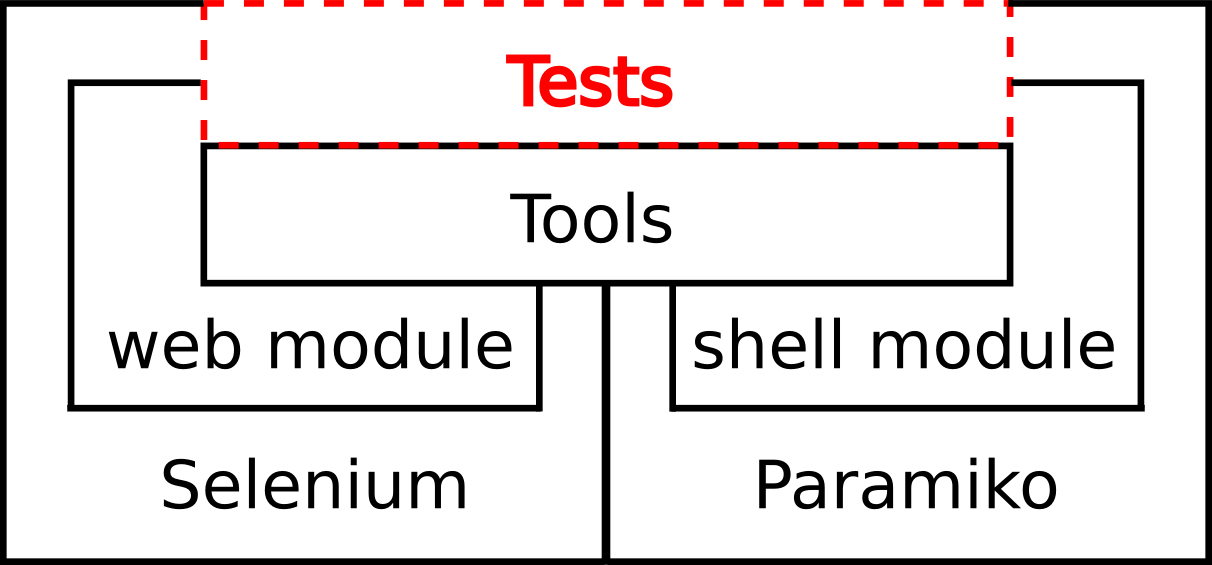
\includegraphics[width=0.5\textwidth]
    {../../images/hubcheck_block_diagram/hubcheck_library_overview_tests.png}
  \caption{ One of HUBcheck's most used features is its test runner and its %
            ability to be embedded within tests. }
  \label{fig:hubzero_library_overview_tests}
\end{figure}

HUBcheck provides the \xfprogramname{hctestrunner} tool to manage the
collection and execution of test cases.  Under the hood,
\xfprogramname{hctestrunner} depends on \xfprogramname{pytest}, a flexible
Python based test case management library that can handle test cases written in
a number of formats including \xfmodule{unittest} \cite{unittest:2015:Online},
\xfmodule{nose} \cite{nose:2015:Online}, and \xfmodule{doctest}
\cite{doctest:2015:Online}.  Section
\ref{sec:building_hubcheck_backed_applications} explored writing programs using
the HUBcheck library, and while test cases can also be written in the same way,
this approach can lead to an excess of code and resource repetition between
test cases. In the following sections, we describe ways to write robust, easy
to understand test cases using the HUBcheck library.

\subsection{Test Fixtures}
\label{ssec:hubcheck_tests_fixtures}

One of the strengths of the \xfprogramname{pytest} library is its flexibility.  Many
test case management libraries include a feature often referred to as a
\textit{test fixture} \cite{TestFixture:Online}.  Test fixtures are functions,
or bits of code, that place the software under test in a fixed state as a
baseline for running tests.

% show example test case noting what would be considered setup and teardown.

Traditionally, x-unit \cite{Xunit:Online} based testing libraries have provided
two types of fixtures: setup fixtures run before a test case, and teardown
fixtures run after the test case. \xfprogramname{pytest} provides a number of
different fixture options which can call upon each other or be reused within
the class, module, or project scopes.

% show example test case using multiple pytest fixtures use different colored
% ablocks to show how fixtures are called before and after a test case

\subsection{The TestCase2 Class}
\label{ssec:hubcheck_tests_testcase2}

HUBcheck provides the \xfclass{TestCase2} class whose purpose is similar to that
of the \xfclass{Tool} class mentioned in Section \ref{ssec:building_a_tool}.
The \xfclass{TestCase2} class provides much of the environment setup and
teardown code needed to run a test and document its behavior in a more detailed
manner than just pass or fail.  The \xfclass{TestCase2} class is responsible for
setting up the filename for browser screenshots, recording individual test
cases to separate video files, setting up test case testdata in local
variables, and managing the page object catalog.  The class also initializes a
local web browser object for each test case.  The \xfclass{TestCase2} class
provides each test case with the following local variables:

\begin{enumerate}
\item \xfparameter{self.browser}
\item \xfparameter{self.catalog}
\item \xfparameter{self.utils}
\item \xfparameter{self.testdata}
\item \xfparameter{self.locators}
\item \xfparameter{self.https\_uri}
\item \xfparameter{self.https\_authority}
\item \xfparameter{self.http\_authority}
\end{enumerate}

\xfclass{TestCase2} hooks into \xfmodule{pytest}'s \xfmethod{setup\_method()} and
\xfmethod{teardown\_method()} test fixtures to provide features similar to that
of HUBcheck based tools.

\subsection{Building a Test Case}
\label{ssec:hubcheck_tests_building}

Consider rewriting the hub website login example, from
\Cref{lst:hubcheck_utils_login}, as a test case.
\Cref{lst:hub_website_login_testcase} demonstrates how to setup a
\xfclass{TestCase2} based test case.  Just like the \xfclass{Tool} class, to use
the \xfclass{TestCase2} class the user first subclasses it.  All classes
derived from \xfclass{TestCase2} have \xfmethod{setup\_method()} and
\xfmethod{teardown\_method()} fixtures, even if it is not explicitly stated in
the derived class as is the case for the \xfmethod{TestHubLogin} class from
\Cref{lst:hub_website_login_testcase}. These two fixtures allow
\xfclass{TestCase2} to perform its variable, browser, page object catalog, and
utility setup before the test case is run, and teardown after the test case has
completed.  In accordance with \xfmodule{pytest}'s test case naming conventions,
all methods of the derived class with names prefixed by \textit{test\_} are
considered test cases.  In \Cref{lst:hub_website_login_testcase}, this
includes the \xfmethod{test\_website\_login()} method.  The test case performs
four tasks.  First, it grabs a username and password from the testdata file in
line 4. Next, it navigates the web browser to the hub's homepage in line 8. In
Line 10, it submits a populated hub login form. Lastly, in line 14, it checks
that the login was successful.


\begin{xcode}{%
  language=python,%
  label=lst:hub_website_login_testcase,%
  caption={Hub website login using HUBcheck's TestCase2 class}%
}
class TestHubLogin(hubcheck.TestCase2):
    def test_website_login(self):
        """ try to login to the hub website """
        self.username,self.userpass = \
            self.testdata.find_account_for('registeredworkspace')

        # setup a web browser
        self.browser.get(self.https_authority)

        self.utils.account.login_as(self.username,self.userpass)

        # verify you have successfully logged in
        po = self.catalog.load_pageobject('GenericPage')
        assert po.header.is_logged_in(),'Login Failed'
\end{xcode}


It is interesting to note how clean and easy to read the
\xfmethod{test\_website\_login()} test case is when compared to the login script
in \Cref{lst:hubcheck_hubzero_login} or even the original login script
in \Cref{lst:selenium_ide_hubzero_login}. Part of the test case's
simplicity is due to its use of the \xfclass{TestCase2} class, which wraps up
most of the standard code needed to setup and teardown the web browser, browser
recording, testdata, page object catalog, and utilities.  Test cases that are
easy to read are often easy to understand and maintain. The \xfclass{TestCase2}
class helps keep test cases short and to the point.

Adding more test cases to the \xfclass{TestHubLogin} class is also easy and
helps demonstrate the power of \xfmodule{pytest}'s fixtures. A complementary
test to logging into the website is logging out. As you might have suspected,
there is a bit of code overlap between the login and logout tests. For example,
in order to test login and logout, both tests need to login.  This common code
can be placed in the \xfmethod{setup\_method()} fixture. In
\Cref{lst:testcase_setup_method}, the code to retrieve the test user
credentials, navigate the browser to the hub's homepage, and login has been
abstracted out of the \xfmethod{test\_website\_login()} test case, and placed
in the \xfclass{TestHubLogin} class's \xfmethod{setup\_method()} fixture. This
fixture and \xfclass{TestCase2}'s \xfmethod{setup\_method()} fixture don't
collide as they would in a normal inheritance situation.  Instead, through the
magic of metaclasses, \xfclass{TestCase2} recognizes the existence of
\xfclass{TestHubLogin}'s \xfmethod{setup\_method()} method, and embeds the
method inside of its \xfmethod{setup\_method()} fixture.  By the time
\xfclass{TestHubLogin}'s \xfmethod{setup\_method()} is called,
\xfclass{TestCase2} has already completed setting up the environment and
variables for the test case. This same embedding happens with
\xfclass{TestHubLogin}'s \xfmethod{teardown\_method()}, but in reverse.
\xfclass{TestCase2} recognizes \xfclass{TestHubLogin}'s
\xfmethod{teardown\_method()} method, calls the method, and then proceeds to
calling its own \xfmethod{teardown\_method()} fixture.

\begin{xcode}{%
  language=python,%
  label=lst:testcase_setup_method,%
  caption={Using pytest fixtures while subclassing the TestCase2 class}%
}
class TestHubLogin(hubcheck.TestCase2):
    def setup_method(self,method):
        self.username,self.userpass = \
            self.testdata.find_account_for('registeredworkspace')

        # setup a web browser
        self.browser.get(self.https_authority)

        # login to the hub website
        self.utils.account.login_as(self.username,self.userpass)
\end{xcode}


% FIXME:
% add a picture of the TestCase2 metaclass wrapping the TestHubLogin's
% setup_method and teardown_method fixtures.

With the \xfmethod{setup\_method()} fixture in place, the new
\xfmethod{test\_website\_login()} test case is even more compact and to the
point. After the \xfmethod{setup\_method()} fixture runs and logs the user into
the hub website, the \xfmethod{test\_website\_login()} test case just checks to
see if the user has successfully logged in.
\Cref{lst:testcase_new_website_login} shows the new
\xfmethod{test\_website\_login()} test case.


\begin{xcode}{%
  language=python,%
  label=lst:testcase_new_website_login,%
  caption={New website login test case, using the setup\_method() fixture}%
}
class TestHubLogin(hubcheck.TestCase2):
    ...
    def test_website_login(self):
        """ try to login to the hub website """
        # verify you have successfully logged in
        po = self.catalog.load_pageobject('GenericPage')
        assert po.header.is_logged_in(),'Login Failed'
\end{xcode}


Similarly, the new \xfmethod{test\_website\_logout()} test case, in
\Cref{lst:testcase_new_website_logout}, verifies that the login was successful,
then attempts to logout of the website. Finally, it checks that logging out of
the website was successful.


\begin{xcode}{%
  language=python,%
  label=lst:testcase_new_website_logout,%
  caption={New website logout test case, using the setup\_method() fixture}%
}
class TestHubLogin(hubcheck.TestCase2):
    ...
    def test_website_logout(self):
        """ try to logout of the hub website """
        # verify you have successfully logged in
        po = self.catalog.load_pageobject('GenericPage')
        assert po.header.is_logged_in(),'Login Failed'

        # logout of the website
        po.header.goto_logout()
        assert not po.header.is_logged_in(),'Logout Failed'
\end{xcode}


Writing test cases using the HUBcheck library is an extension of writing
programs that use the library. Many features are analogous, including setting
up the environment, starting the web browser, starting a web proxy, setting up
a recordable virtual framebuffer, and loading testdata. Much of the boilerplate
code for setup and teardown is taken care of by the
\xfprogramname{hctestrunner} tool and the \xfclass{TestCase2} class. When used
together, developers are able to quickly write easy to read, robust test cases.

\subsection{HUBcheck's Test Suites}
\label{ssec:hubcheck_tests_suites}

Test cases can be grouped into test suites by using a feature from
\xfprogramname{pytest} called \textit{marks}.  \xfprogramname{pytest} marks are
a way of tagging or marking tests.  \xfprogramname{pytest} provides an easy way
to collect all tests with a specific mark or a logical combination of marks
using the \xfparameter{-m} flag.  Tests that come with the HUBcheck library are
tagged with at least one of several popular marks that denote when the test
should be run including \textit{nightly}, \textit{weekly}, \textit{upgrade},
\textit{prod\_safe\_upgrade}, \textit{reboot}, and \textit{hcunit}.
